


%_______________
\section{Exercises}



%_______________
\subsection{Variability in estimates}

% 1

\eoce{\qt{Identify the parameter, Part I\label{identify_parameter_1}} For each of the following situations, state 
whether the parameter of interest is a mean or a proportion. It may be helpful 
to examine whether individual responses are numerical or categorical.
\begin{parts}
\item In a survey, one hundred college students are asked how many hours per 
week they spend on the Internet.
\item In a survey, one hundred college students are asked: ``What percentage of 
the time you spend on the Internet is part of your course work?"
\item In a survey, one hundred college students are asked whether or not they 
cited information from Wikipedia in their papers.
\item In a survey, one hundred college students are asked what percentage of 
their total weekly spending is on alcoholic beverages.
\item In a sample of one hundred recent college graduates, it is found that 85 
percent expect to get a job within one year of their graduation date.
\end{parts}
}{}

% 2

\eoce{\qt{Identify the parameter, Part II\label{identify_parameter_2}} For each of the 
following situations, state whether the parameter of interest is a mean or a 
proportion. 
\begin{parts}
\item A poll shows that 64\% of Americans personally worry a great deal about 
federal spending and the budget deficit.
\item A survey reports that local TV news has shown a 17\% increase in revenue 
between 2009 and 2011 while newspaper revenues decreased by 6.4\% during this 
time period.
\item In a survey, high school and college students are asked whether or not 
they use geolocation services on their smart phones.
\item In a survey, smart phone users are asked whether or not they use a web-based taxi service.
\item In a survey, smart phone users are asked how many times they used a web-based taxi service over the last year.
\end{parts}
}{}

\textC{\newpage}

% 3

\eoce{\qt{College credits\label{college_credits}} A college counselor is interested in 
estimating how many credits a student typically enrolls in each semester. The 
counselor decides to randomly sample 100 students by using the registrar's 
database of students. The histogram below shows the distribution of the number 
of credits taken by these students. Sample statistics for this distribution are 
also provided.\\
\begin{minipage}[c]{0.75\textwidth}
\begin{center}
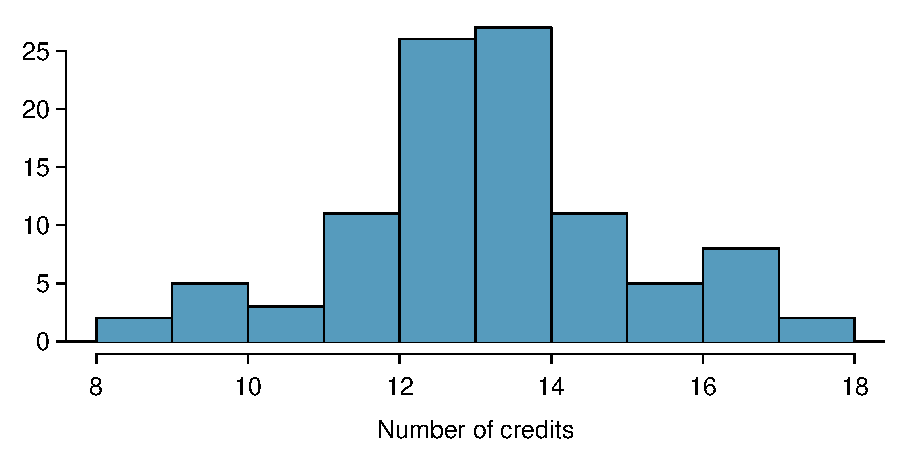
\includegraphics[width=\textwidth]{ch_inference_foundations/figures/eoce/college_credits/college_credits_hist.pdf}
\end{center}
\end{minipage}
\begin{minipage}[c]{0.22\textwidth}
\begin{center}
\begin{tabular}{l|r l}
Min     & 8 \\
Q1      & 13 \\
Median  & 14 \\
Mean    & 13.65 \\
SD      & 1.91 \\
Q3      & 15 \\
Max     & 18 \\
\end{tabular}
\end{center}
\end{minipage}
\begin{parts}
\item What is the point estimate for the average number of credits taken per 
semester by students at this college? What about the median?
\item What is the point estimate for the standard deviation of the number of 
credits taken per semester by students at this college? What about the IQR?
\item Is a load of 16 credits unusually high for this college? What about 18 
credits? Explain your reasoning. \textit{Hint:} Observations farther than two 
standard deviations from the mean are usually considered to be unusual.
\item The college counselor takes another random sample of 100 students and this 
time finds a sample mean of 14.02 units. Should she be surprised that this 
sample statistic is slightly different than the one from the original sample? 
Explain your reasoning.
\item The sample means given above are point estimates for the mean number of 
credits taken by all students at that college. What measures do we use to 
quantify the variability of this estimate (Hint: recall that 
$SD_{\bar{x}} = \frac{\sigma}{\sqrt{n}}$)? Compute this quantity using the data 
from the original sample.
\end{parts}
}{}

% 4

\eoce{\qt{Heights of adults\label{adult_heights}} Researchers studying anthropometry 
collected body girth measurements and skeletal diameter measurements, as well as 
age, weight, height and gender, for 507 physically active individuals. The 
histogram below shows the sample distribution of heights in centimeters. 
\footfullcite{Heinz:2003} \\
\begin{minipage}[c]{0.75\textwidth}
\begin{center}
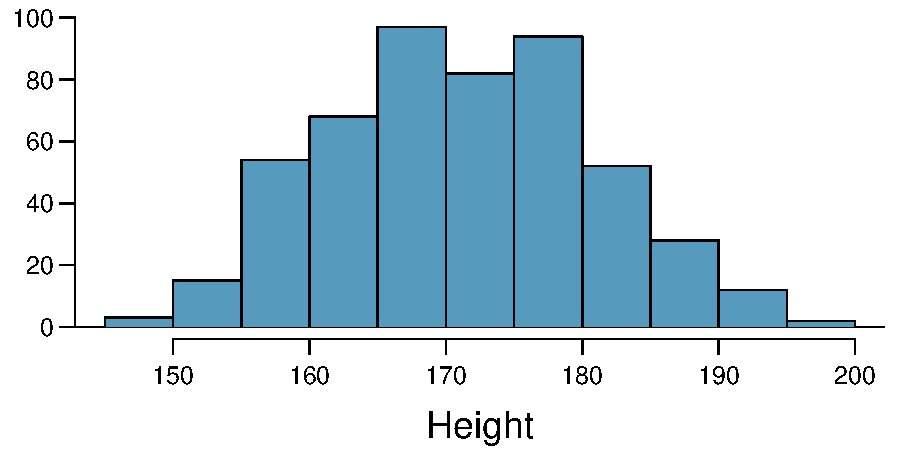
\includegraphics[width=\textwidth]{ch_inference_foundations/figures/eoce/adult_heights/adult_heights_hist.pdf}
\end{center}
\end{minipage}
\begin{minipage}[c]{0.23\textwidth}
\begin{center}
\begin{tabular}{l|r l}
Min     & 147.2 \\
Q1      & 163.8 \\
Median  & 170.3 \\
Mean    & 171.1 \\
SD      &  9.4 \\
Q3      & 177.8 \\
Max     & 198.1 \\
\end{tabular}
\end{center}
\end{minipage}
\begin{parts}
\item What is the point estimate for the average height of active individuals? 
What about the median?
\textC{\textbf{(See the next page for parts~(b)-(e).)}}
\item What is the point estimate for the standard deviation of the heights of 
active individuals? What about the IQR?
\item Is a person who is 1m 80cm (180 cm) tall considered unusually tall? And is 
a person who is 1m 55cm (155cm) considered unusually short? Explain your 
reasoning.
\item The researchers take another random sample of physically active 
individuals. Would you expect the mean and the standard deviation of this new 
sample to be the ones given above? Explain your reasoning.
\item The sample means obtained are point estimates for the mean height of all 
active individuals, if the sample of individuals is equivalent to a simple 
random sample. What measure do we use to quantify the variability of such an 
estimate (Hint: recall that $SD_{\bar{x}} = \frac{\sigma}{\sqrt{n}}$)? Compute 
this quantity using the data from the original sample under the condition that 
the data are a simple random sample. 
\end{parts}
}{}

% 5

\eoce{\qt{Hen eggs\label{hen_eggs}} The distribution of the number of eggs laid 
by a certain species of hen during their breeding period has a mean of 35 eggs 
with a standard deviation of 18.2. Suppose a group of researchers 
randomly samples 45 hens of this species, counts the number of eggs laid 
during their breeding period, and records the sample mean. They repeat 
this 1,000 times, and build a distribution of sample 
means. 
\begin{parts}
\item What is this distribution called? 
\item Would you expect the shape of this distribution to be symmetric, right 
skewed, or left skewed? Explain your reasoning.
\item Calculate the variability of this distribution and state the appropriate 
term used to refer to this value.
\item Suppose the researchers' budget is reduced and they are only able to 
collect random samples of 10 hens. The sample mean of the number of eggs is 
recorded, and we repeat this 1,000 times, and build a new distribution of sample 
means. How will the variability of this new distribution compare to the 
variability of the original distribution?
\end{parts}
}{}

% 6

\eoce{\qt{Art after school\label{art_after_school}} Elijah and Tyler, 
two high school juniors, conducted a survey on 15 students at their school, 
asking the students whether they would like the school to offer an 
after-school art program, counted the number of ``yes" answers, and 
recorded the sample proportion. 14 out of the 15 students responded 
``yes". They repeated this 100 times and built a distribution of 
sample means.
(Note that this question requires having reviewed
Section~\ref{normalApproxBinomialDistSubsection}
on the normal approximation to the binomial distribution.)
\begin{parts}
\item What is this distribution called? 
\item Would you expect the shape of this distribution to be symmetric, right 
skewed, or left skewed? Explain your reasoning.
\item Calculate the variability of this distribution and state the appropriate 
term used to refer to this value.
\item Suppose that the students were able to recruit a few more friends to help 
them with sampling, and are now able to collect data from random samples of 25 
students. Once again, they record the number of ``yes" answers, and record the 
sample proportion, and repeat this 100 times to build a new distribution of 
sample proportions. How will the variability of this new distribution compare to 
the variability of the original distribution?
\end{parts}
}{}


\textC{\newpage}


%_______________
\subsection{Confidence intervals}

% 7

\eoce{\qt{Chronic illness, Part I\label{chronic_illness_intro}} 
In 2013, the Pew Research Foundation reported that ``45\% of U.S. adults report 
that they live with one or more chronic conditions''.
\footfullcite{data:pewdiagnosis:2013} However, this value was based on a sample, 
so it may not be a perfect estimate for the population parameter of interest on 
its own. The study reported a standard error of about 1.2\%, and a normal model 
may reasonably be used in this setting. Create a 95\% confidence interval for 
the proportion of U.S. adults who live with one or more chronic conditions. Also 
interpret the confidence interval in the context of the study.
}{}

% 8

\eoce{\qt{Twitter users and news, Part I\label{twitter_users_intro}} 
A poll conducted in 2013 found that 52\% of U.S. adult Twitter users 
get at least some news on Twitter.\footfullcite{data:pewtwitternews:2013}. 
The standard error for this estimate was 2.4\%, and a normal distribution 
may be used to model the sample proportion. Construct a 99\% confidence 
interval for the fraction of U.S. adult Twitter users who get some 
news on Twitter, and interpret the confidence interval in context.
}{}

% 9

\eoce{\qt{Chronic illness, Part II\label{chronic_illness_tf}} In 2013, the Pew Research Foundation reported that 
``45\% of U.S. adults report that they live with one or more chronic 
conditions'', and the standard error for this estimate is 1.2\%. Identify each 
of the following statements as true or false. Provide an explanation to justify 
each of your answers.
\begin{parts}
\item We can say with certainty that the confidence interval from 
Exerise~\ref{chronic_illness_intro} contains the true percentage of U.S. adults who 
suffer from a chronic illness.
\item If we repeated this study 1,000 times and constructed a 95\% confidence 
interval for each study, then approximately 950 of those confidence intervals 
would contain the true fraction of U.S. adults who suffer from chronic illnesses.
\item The poll provides statistically significant evidence (at the 
$\alpha = 0.05$ level) that the percentage of U.S. adults who suffer from 
chronic illnesses is below 50\%.
\item Since the standard error is 1.2\%, only 1.2\% of people in the study 
communicated uncertainty about their answer.
\end{parts}
}{}

% 10

\eoce{\qt{Twitter users and news, Part II\label{twitter_users_tf}} A poll conducted in 2013 found that 52\% of 
U.S. adult Twitter users get at least some news on Twitter, and the standard 
error for this estimate was 2.4\%. Identify each of the following statements as 
true or false. Provide an explanation to justify each of your answers.
\begin{parts}
\item The data provide statistically significant evidence that more than half of 
U.S. adult Twitter users get some news through Twitter. Use a significance level 
of $\alpha = 0.01$.
\item Since the standard error is 2.4\%, we can conclude that 97.6\% of all U.S. 
adult Twitter users were included in the study.
\item If we want to reduce the standard error of the estimate, we should collect 
less data.
\item If we construct a 90\% confidence interval for the percentage of U.S. 
adults Twitter users who get some news through Twitter, this confidence interval 
will be wider than a corresponding 99\% confidence interval.
\end{parts}
}{}

\textC{\newpage}

% 11

\eoce{\qt{Relaxing after work\label{relax_after_work}} The 2010 General Social Survey asked the question:
``After an average work day, about how many hours do you have to relax or pursue 
activities that you enjoy?" to a random sample of 1,155 Americans.\footfullcite{data:gss:2010} A 95\% confidence interval for the mean number of hours spent 
relaxing or pursuing activities they enjoy was (1.38, 1.92).
\begin{parts}
\item Interpret this interval in context of the data.
\item Suppose another set of researchers reported a confidence interval with a 
larger margin of error based on the same sample of 1,155 Americans. How does 
their confidence level compare to the confidence level of the interval stated 
above?
\item Suppose next year a new survey asking the same question is conducted, and 
this time the sample size is 2,500. Assuming that the population 
characteristics, with respect to how much time people spend relaxing after work, 
have not changed much within a year. How will the margin of error of the 95\% 
confidence interval constructed based on data from the new survey compare to the 
margin of error of the interval stated above?
\end{parts}
}{}

% 12

\eoce{\qt{Mental health\label{mental_health}} The 2010 General Social Survey asked the question: ``For how many days during the past 30 days was your 
mental health, which includes stress, depression, and problems with emotions, 
not good?" Based on responses from 1,151 US residents, the survey reported a 95\%
 confidence interval of 3.40 to 4.24 days in 2010.
\begin{parts}
\item Interpret this interval in context of the data.
\item What does ``95\% confident" mean? Explain in the context of the application.
\item Suppose the researchers think a 99\% confidence level would be more 
appropriate for this interval. Will this new interval be smaller or larger than 
the 95\% confidence interval?
\item If a new survey were to be done with 500 Americans, would the standard 
error of the estimate be larger, smaller, or about the same. Assume the standard 
deviation has remained constant since 2010.
\end{parts}
}{}

% 13

\eoce{\qt{Waiting at an ER, Part I\label{er_wait_intro}} A hospital administrator 
hoping to improve wait times decides to estimate the average emergency 
room waiting time at her hospital. She collects a simple random sample 
of 64 patients and determines the time (in minutes) between when they 
checked in to the ER until they were first seen by a doctor. A 95\% 
confidence interval based on this sample is (128 minutes, 147 minutes), 
which is based on the normal model for the mean. Determine whether the 
following statements are true or false, and explain your reasoning.
\begin{parts}
\item This confidence interval is not valid since we do not know if the 
population distribution of the ER wait times is nearly Normal.
\item We are 95\% confident that the average waiting time of these 64 emergency 
room patients is between 128 and 147 minutes.
\item We are 95\% confident that the average waiting time of all patients at 
this hospital's emergency room is between 128 and 147 minutes.
\item 95\% of random samples have a sample mean between 128 and 147 minutes.
\item A 99\% confidence interval would be narrower than the 95\% confidence 
interval since we need to be more sure of our estimate.
\item The margin of error is 9.5 and the sample mean is 137.5.
\item In order to decrease the margin of error of a 95\% confidence interval to 
half of what it is now, we would need to double the sample size.
\end{parts}
}{}

\textC{\newpage}

% 14

\eoce{\qt{Thanksgiving spending, Part I\label{thanksgiving_spending_intro}} 
The 2009 holiday retail season, which kicked off on November 27, 2009 
(the day after Thanksgiving), had been marked by somewhat lower 
self-reported consumer spending than was seen during the comparable 
period in 2008. To get an estimate of consumer spending, 436 randomly 
sampled American adults were surveyed. Daily consumer spending for the 
six-day period after Thanksgiving, spanning the Black Friday weekend and 
Cyber Monday, averaged \$84.71. A 95\% confidence interval based on 
this sample is (\$80.31, \$89.11). Determine whether the following 
statements are true or false, and explain your reasoning.
\begin{center}
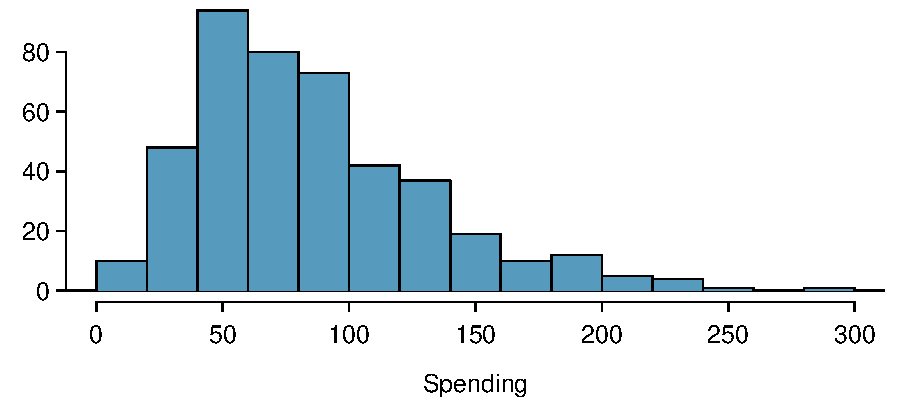
\includegraphics[width=100mm]{ch_inference_foundations/figures/eoce/thanksgiving_spending_intro/thanksgiving_spending_intro_pop_hist.pdf}
\end{center}
\begin{parts}
\item We are 95\% confident that the average spending of these 436 American 
adults is between \$80.31 and \$89.11.
\item This confidence interval is not valid since the distribution of spending 
in the sample is right skewed.
\item 95\% of random samples have a sample mean between \$80.31 and \$89.11.
\item We are 95\% confident that the average spending of all American adults is 
between \$80.31 and \$89.11.
\item A 90\% confidence interval would be narrower than the 95\% confidence 
interval since we don't need to be as sure about our estimate.
\item In order to decrease the margin of error of a 95\% confidence interval to 
a third of what it is now, we would need to use a sample 3 times larger.
\item The margin of error is 4.4.
\end{parts}
}{}

% 15

\eoce{\qt{Exclusive relationships\label{exclusive_relationships}} A survey conducted 
on a reasonably random sample of 203 undergraduates asked, among many other 
questions, about the number of exclusive relationships these students have been 
in. The histogram below shows the distribution of the data from this sample. 
The sample average is 3.2 with a standard deviation of 1.97.
\begin{center}
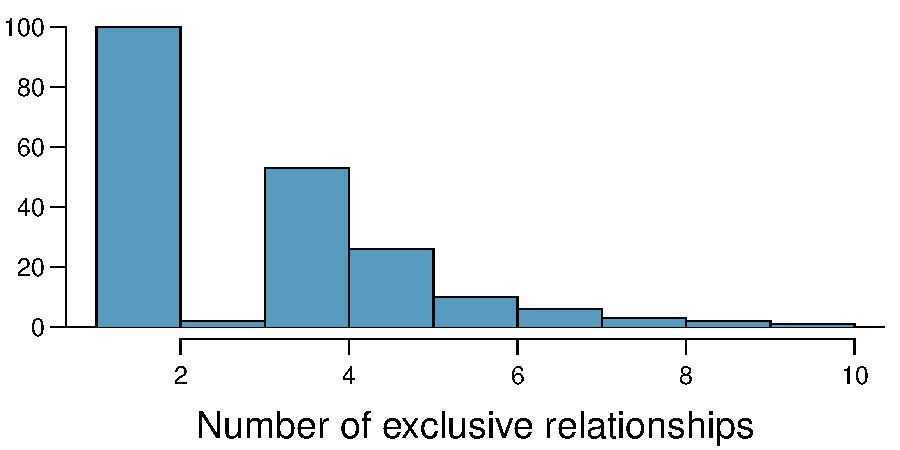
\includegraphics[width=0.6\textwidth]{ch_inference_foundations/figures/eoce/exclusive_relationships/exclusive_relationships_rel_hist.pdf}
\end{center}
Estimate the average number of exclusive relationships Duke students have been 
in using a 90\% confidence interval and interpret this interval in context. 
Check any conditions required for inference, and note any assumptions you must 
make as you proceed with your calculations and conclusions.
}{}

% 16

\eoce{\qt{Age at first marriage, Part I\label{age_at_first_marriage_intro}} 
The National Survey of Family Growth conducted by the Centers for Disease 
Control gathers information on family life, marriage and divorce, pregnancy, 
infertility, use of contraception, and men's and women's health. One of the 
variables collected on this survey is the age at first marriage. The histogram 
below shows the distribution of ages at first marriage of 5,534 randomly sampled 
women between 2006 and 2010. The average age at first marriage among these women 
is 23.44 with a standard deviation of 4.72.\footfullcite{data:nsfg:2010}
\begin{center}
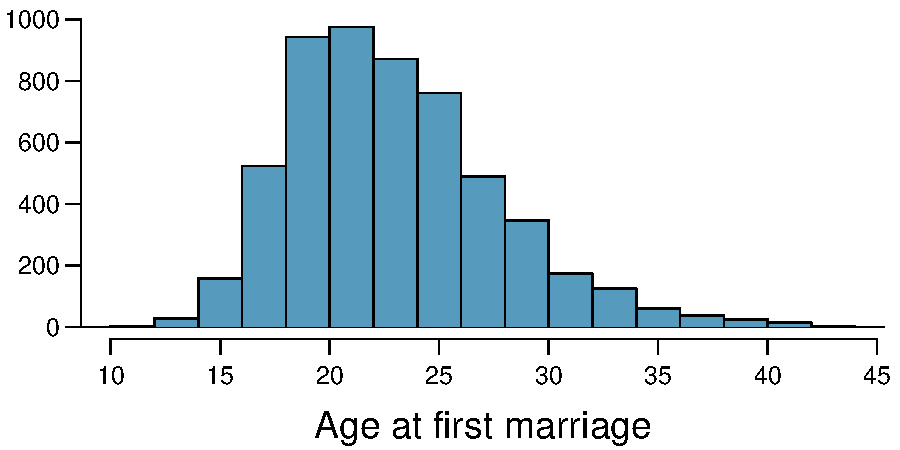
\includegraphics[width=0.6\textwidth]{ch_inference_foundations/figures/eoce/age_at_first_marriage_intro/age_at_first_marriage_intro_hist.pdf}
\end{center}
Estimate the average age at first marriage of women using a 95\% confidence 
interval, and interpret this interval in context. Discuss any relevant 
assumptions.
}{}



%_______________
\subsection{Hypothesis testing}

% 17

\eoce{\qt{Identify hypotheses, Part I\label{identify_hypotheses_1}} Write the null 
and alternative hypotheses in words and then symbols for each of the following 
situations.
\begin{parts}
\item New York is known as ``the city that never sleeps". A random sample of 25 
New Yorkers were asked how much sleep they get per night. Do these data provide 
convincing evidence that New Yorkers on average sleep less than 8 hours a night?
\item Employers at a firm are worried about the effect of March Madness, a 
basketball championship held each spring in the US, on employee productivity. 
They estimate that on a regular business day employees spend on average 15 
minutes of company time checking personal email, making personal phone calls, 
etc. They also collect data on how much company time employees spend on such non-
business activities during March Madness. They want to determine if these data 
provide convincing evidence that employee productivity decreases during March 
Madness.
\end{parts}
}{}

% 18

\eoce{\qt{Identify hypotheses, Part II\label{identify_hypotheses_2}} 
Write the null and alternative hypotheses in words and using symbols 
for each of the following situations.
\begin{parts}
\item Since 2008, chain restaurants in California have been required to display 
calorie counts of each menu item. Prior to menus displaying calorie counts, the 
average calorie intake of diners at a restaurant was 1100 calories. After 
calorie counts started to be displayed on menus, a nutritionist collected data 
on the number of calories consumed at this restaurant from a random sample of 
diners. Do these data provide convincing evidence of a difference in the average 
calorie intake of a diners at this restaurant?
\item Based on the performance of those who took the GRE exam between July 1, 
2004 and June 30, 2007, the average Verbal Reasoning score was calculated to be 
462. In 2011 the average verbal score was slightly higher. Do these data provide 
convincing evidence that the average GRE Verbal Reasoning score has changed 
since 2004?
\end{parts}
}{}

\textC{\pagebreak}

% 19

\eoce{\qt{Online communication\label{online_communication}} A study suggests that the 
average college student spends 10 hours per week communicating with others 
online. You believe that this is an underestimate and decide to collect your 
own sample for a hypothesis test. You randomly sample 60 students from your 
dorm and find that on average they spent 13.5 hours a week communicating with 
others online. A friend of yours, who offers to help you with the hypothesis 
test, comes up with the following set of hypotheses. Indicate any errors you see.
\begin{align*}
H_0&: \bar{x} < 10~hours \\
H_A&: \bar{x} > 13.5~hours
\end{align*}
}{}

% 20

\eoce{\qt{Age at first marriage, Part II\label{age_at_first_marriage_hyp_errors}} Exercise~\ref{age_at_first_marriage_intro} presents the results 
of a 2006 - 2010 survey showing that the average age of women at first marriage 
is 23.44. Suppose a social scientist believes that this value has increased in 
2012, but she would also be interested if she found a decrease. Below is how she 
set up her hypotheses. Indicate any errors you see.
\begin{align*}
H_0&: \bar{x} = 23.44~years~old \\
H_A&: \bar{x} > 23.44~years~old
\end{align*}
}{}

% 21

\eoce{\qt{Waiting at an ER, Part II\label{er_wait_ci_ht}} Exercise~\ref{er_wait_intro} 
provides a 95\% confidence interval for the mean waiting time at an emergency 
room (ER) of (128 minutes, 147 minutes). Answer the following questions based on
this interval.
\begin{parts}
\item A local newspaper claims that the average waiting time at this ER exceeds 
3 hours. Is this claim supported by the confidence interval? Explain your 
reasoning.
\item The Dean of Medicine at this hospital claims the average wait time is 2.2 
hours. Is this claim supported by the confidence interval? Explain your 
reasoning.
\item Without actually calculating the interval, determine if the claim of the 
Dean from part (b) would be supported based on a 99\% confidence interval?
\end{parts}
}{}

% 22

\eoce{\qt{Thanksgiving spending, Part II\label{thanksgiving_spending_ht}} 
Exercise~\ref{thanksgiving_spending_intro} provides a 95\% confidence interval 
for the average spending by American adults during the six-day period 
after Thanksgiving 2009: 
(\$80.31, \$89.11). 
\begin{parts}
\item A local news anchor claims that the average spending during this period in 
2009 was \$100. What do you think of her claim?
\item Would the news anchor's claim be considered reasonable based on a 90\% 
confidence interval? Why or why not? (Do not actually calculate the interval.)
\end{parts}
}{}

% 23

\eoce{\qt{Nutrition labels\label{nutrition_labels}} The nutrition label on a bag of 
potato chips says that a one ounce (28~gram) serving of potato chips has 130 
calories and contains ten grams of fat, with three grams of saturated fat. A 
random sample of 35 bags yielded a sample mean of 134 calories with a standard 
deviation of 17 calories. Is there evidence that the nutrition label does not 
provide an accurate measure of calories in the bags of potato chips? We have 
verified the independence, sample size, and skew conditions are satisfied.
}{}

\textC{\newpage}

% 24

\eoce{\qt{Gifted children, Part I\label{gifted_children_intro}} Researchers 
investigating characteristics of gifted children collected data from schools 
in a large city on a random sample of thirty-six children who were identified 
as gifted children soon after they reached the age of four. The following 
histogram shows the distribution of the ages (in months) at which these 
children first counted to 10 successfully. Also provided are some sample 
statistics.\footfullcite{Graybill:1994}

\begin{center}
\begin{minipage}[c]{0.6\textwidth}
\begin{center}
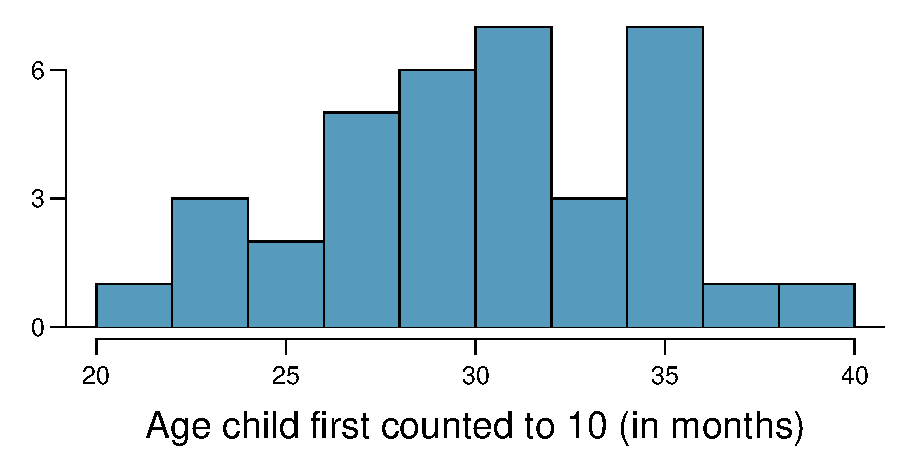
\includegraphics[width=\textwidth]{ch_inference_foundations/figures/eoce/gifted_children_intro/gifted_children_ht_count_hist.pdf} 
\end{center}
\end{minipage}
\begin{minipage}[c]{0.1\textwidth}
\begin{tabular}{r | l}
n   & 36 \\
min & 21 \\
mean    & 30.69 \\
sd  & 4.31 \\
max & 39 
\end{tabular}
\end{minipage}
\end{center}

\begin{parts}
\item Are conditions for inference satisfied?
\item Suppose you read online that children first count to 10 successfully when 
they are 32 months old, on average. Perform a hypothesis test to evaluate if 
these data provide convincing evidence that the average age at which gifted 
children first count to 10 successfully is less than the general average of 32 
months. Use a significance level of 0.10.
\item Interpret the p-value in context of the hypothesis test and the data. 
\item Calculate a 90\% confidence interval for the average age at which gifted children first count to 10 successfully.
\item Do your results from the hypothesis test and the confidence interval agree? Explain.
\end{parts}
}{}

% 25

\eoce{\qt{Waiting at an ER, Part III\label{er_wait_ht}} The hospital administrator 
mentioned in Exercise~\ref{er_wait_intro} randomly selected 64 patients and 
measured the time (in minutes) between when they checked in to the ER and the 
time they were first seen by a doctor. The average time is 137.5 minutes and 
the standard deviation is 39 minutes. She is getting grief from her supervisor 
on the basis that the wait times in the ER has increased greatly from last 
year's average of 127 minutes. However, she claims that the increase is 
probably just due to chance. 
\begin{parts}
\item Are conditions for inference met? Note any assumptions you must make to 
proceed.
\item Using a significance level of $\alpha = 0.05$, is the change in wait times 
statistically significant? Use a two-sided test since it seems the supervisor 
had to inspect the data before she suggested an increase occurred.
\item Would the conclusion of the hypothesis test change if the significance 
level was changed to $\alpha = 0.01$?
\end{parts}
}{}

\textC{\newpage}

% 26

\eoce{\qt{Gifted children, Part II\label{gifted_children_ht}} Exercise~\ref{gifted_children_intro} describes a study on gifted 
children. In this study, along with variables on the children, the researchers 
also collected data on the mother's and father's IQ of the 36 randomly sampled 
gifted children. The histogram below shows the distribution of mother's IQ.  
Also provided are some sample statistics.

\begin{center}
\begin{minipage}[c]{0.6\textwidth}
\begin{center}
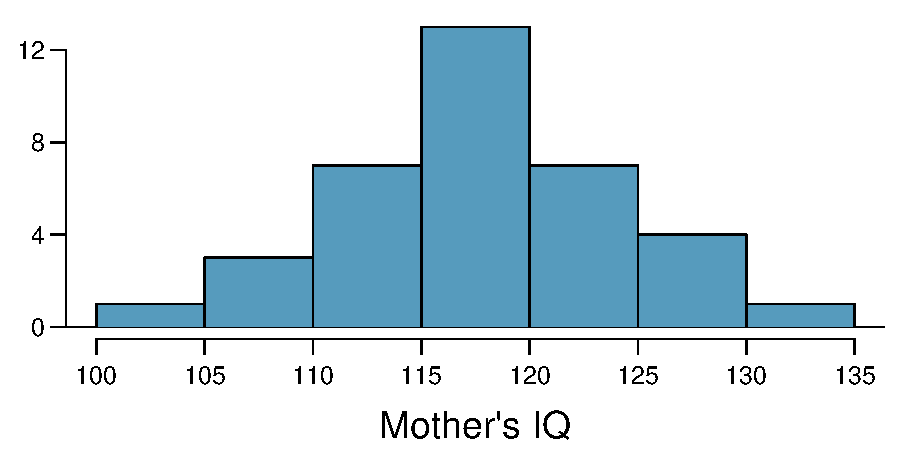
\includegraphics[width=\textwidth]{ch_inference_foundations/figures/eoce/gifted_children_ht/gifted_children_ht_momIQ_hist.pdf} 
\end{center}
\end{minipage}
\begin{minipage}[c]{0.1\textwidth}
\begin{tabular}{r | l}
n   & 36 \\
min & 101 \\
mean    & 118.2 \\
sd  & 6.5 \\
max & 131 
\end{tabular}
\end{minipage}
\end{center}

\begin{parts}
\item Perform a hypothesis test to evaluate if these data provide convincing 
evidence that the average IQ of mothers of gifted children is different than the 
average IQ for the population at large, which is 100. Use a significance level 
of 0.10.
\item Calculate a 90\% confidence interval for the average IQ of mothers of 
gifted children.
\item Do your results from the hypothesis test and the confidence interval 
agree? Explain.
\end{parts}
}{}

% 27

\eoce{\qt{Working backwards, one-sided\label{backwards_one_sided}} You are given the 
following hypotheses:
\begin{align*}
H_0&: \mu = 30 \\
H_A&: \mu > 30
\end{align*}
We know that the sample standard deviation is 10 and the sample size is 70. For 
what sample mean would the p-value be equal to 0.05? Assume that all conditions 
necessary for inference are satisfied.
}{}

% 28

\eoce{\qt{Working backwards, two-sided\label{backwards_two_sided}} You are given the 
following hypotheses:
\begin{align*}
H_0&: \mu = 30 \\
H_A&: \mu \ne 30
\end{align*}
We know that the sample standard deviation is 10 and the sample size is 70. For 
what sample mean would the p-value be equal to 0.05? Assume that all conditions 
necessary for inference are satisfied.
}{}

% 29

\eoce{\qt{Testing for Fibromyalgia\label{errors_fibromyalgia}} A patient named Diana 
was diagnosed with Fibromyalgia, a long-term syndrome of body pain, and was 
prescribed anti-depressants. Being the skeptic that she is, Diana didn't 
initially believe that anti-depressants would help her symptoms. However after 
a couple months of being on the medication she decides that the 
anti-depressants are working, because she feels like her symptoms are in fact 
getting better.
\begin{parts}
\item Write the hypotheses in words for Diana's skeptical position when she 
started taking the anti-depressants.
\item What is a Type~1 Error in this context?
\item What is a Type~2 Error in this context?
\end{parts}
}{}

\textC{\newpage}

% 30

\eoce{\qt{Testing for food safety\label{errors_food_safety}} A food safety inspector 
is called upon to investigate a restaurant with a few customer reports of poor 
sanitation practices. The food safety inspector uses a hypothesis testing 
framework to evaluate whether regulations are not being met. If he decides 
the restaurant is in gross violation, its license to serve food will be revoked.
\begin{parts}
\item Write the hypotheses in words.
\item What is a Type~1 Error in this context?
\item What is a Type~2 Error in this context?
\item Which error is more problematic for the restaurant owner? Why?
\item Which error is more problematic for the diners? Why?
\item As a diner, would you prefer that the food safety inspector requires 
strong evidence or very strong evidence of health concerns before revoking a 
restaurant's license? Explain your reasoning.
\end{parts}
}{}

% 31

\eoce{\qtq{Which is higher\label{which_higher_found_inf}} In each part below, there is a value of interest and two 
scenarios (I and II). For each part, report if the value of interest is larger 
under scenario I, scenario II, or whether the value is equal under the scenarios.
\begin{parts}
\item The standard error of $\bar{x}$ when $s = 120$ and 
(I) n = 25 or (II) n = 125.
\item The margin of error of a confidence interval when the confidence level is 
(I) 90\% or (II) 80\%.
\item The p-value for a Z-statistic of 2.5 when (I) n = 500 or (II) n = 1000.
\item The probability of making a Type~2 Error when the alternative hypothesis 
is true and the significance level is (I) 0.05 or (II) 0.10.
\end{parts}
}{}

% 32

\eoce{\qt{True or false\label{tf_found_inf}} Determine if the following statements are true or false, and 
explain your reasoning. If false, state how it could be corrected.
\begin{parts}
\item If a given value (for example, the null hypothesized value of a parameter) 
is within a 95\% confidence interval, it will also be within a 99\% confidence 
interval.
\item Decreasing the significance level ($\alpha$) will increase the probability 
of making a Type~1 Error.
\item Suppose the null hypothesis is $\mu = 5$ and we fail to reject $H_0$. 
Under this scenario, the true population mean is 5.
\item If the alternative hypothesis is true, then the probability of making a 
Type~2 Error and the power of a test add up to 1.
\item With large sample sizes, even small differences between the null value and 
the true value of the parameter, a difference often called the effect size
\index{effect size}, will be identified as statistically significant.
\end{parts}
}{}


\textC{\newpage}


%_______________
\subsection{Examining the Central Limit Theorem}

% 33

\eoce{\qt{Ages of pennies\label{pennies_ages}} The histogram below shows 
the distribution of ages of pennies at a bank. 
\begin{parts}
\item Describe the distribution.
\item Sampling distributions for means from simple random samples of 5, 30, and 
100 pennies is shown in the histograms below. Describe the shapes of these 
distributions and comment on whether they look like what you would expect to see 
based on the Central Limit Theorem.
\item The mean age of the pennies is 10.44 years, with a standard 
deviation of 9.2 years. Using the Central Limit Theorem, calculate the means and 
standard deviations of the distribution of means from random samples of size 5, 
30, and 100. Comment on whether the sampling distributions shown in part~(b) 
agree with the values you compute.
\end{parts}
\begin{center}
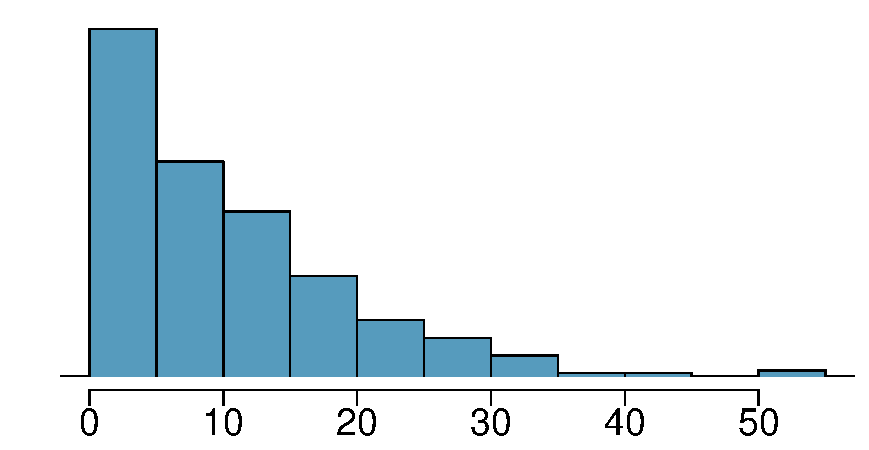
\includegraphics[width=0.6\textwidth]{ch_inference_foundations/figures/eoce/pennies_ages/pennies_ages_pop.pdf} \\
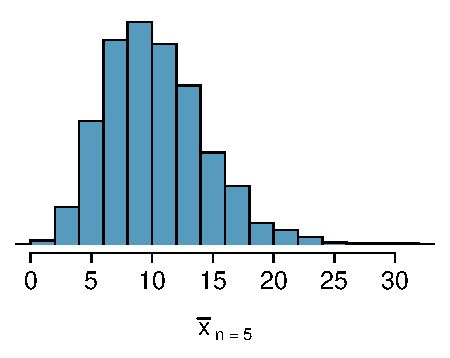
\includegraphics[width=0.325\textwidth]{ch_inference_foundations/figures/eoce/pennies_ages/pennies_ages_sampling_n5.pdf} 
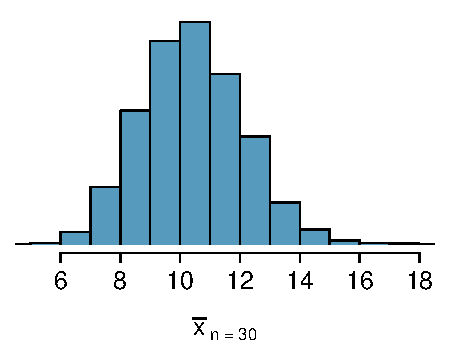
\includegraphics[width=0.325\textwidth]{ch_inference_foundations/figures/eoce/pennies_ages/pennies_ages_sampling_n30.pdf} 
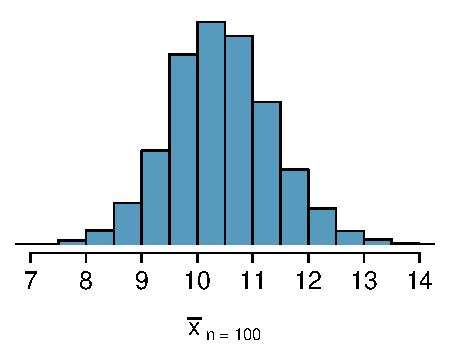
\includegraphics[width=0.325\textwidth]{ch_inference_foundations/figures/eoce/pennies_ages/pennies_ages_sampling_n100.pdf} 
\end{center}
}{}

% 34

\eoce{\qt{CLT\label{CLT}} Define the term ``sampling distribution" of the mean, and describe how the shape, center, and spread of the sampling distribution of the mean change as sample size increases.
}{}

% 35

\eoce{\qt{Housing prices\label{housing_prices}} A housing survey was conducted to 
determine the price of a typical home in Topanga, CA. The mean price of a house 
was roughly \$1.3 million with a standard deviation of \$300,000. There were no 
houses listed below \$600,000 but a few houses above \$3 million.
\begin{parts}
\item Is the distribution of housing prices in Topanga symmetric, right skewed, 
or left skewed? \textit{Hint:} Sketch the distribution.
\item Would you expect most houses in Topanga to cost more or less than \$1.3 
million?
\item Can we estimate the probability that a randomly chosen house in Topanga 
costs more than \$1.4 million using the normal distribution?
\item What is the probability that the mean of 60 randomly chosen houses in 
Topanga is more than \$1.4 million?
\item How would doubling the sample size affect the standard deviation of the 
mean?
\end{parts}
}{}

\textC{\newpage}

% 36

\eoce{\qt{Stats final scores\label{stats_final_scores}} Each year about 1500 students 
take the introductory statistics course at a large university. This year scores 
on the final exam are distributed with a median of 74 points, a mean of 70 
points, and a standard deviation of 10 points. There are no students who scored 
above 100 (the maximum score attainable on the final) but a few students scored 
below 20 points.
\begin{parts}
\item Is the distribution of scores on this final exam symmetric, right skewed, 
or left skewed?
\item Would you expect most students to have scored above or below 70 points?
\item Can we calculate the probability that a randomly chosen student scored 
above 75 using the normal distribution?
\item What is the probability that the average score for a random sample of 40 
students is above 75?
\item How would cutting the sample size in half affect the standard deviation of 
the mean?
\end{parts}
}{}

% 37

\eoce{\qt{Identify distributions, Part I\label{identify_dist_symm_pop}} Four plots 
are presented below. The plot at the top is a distribution for a population. The 
mean is 10 and the standard deviation is 3. Also shown below is a distribution 
of (1) a single random sample of 100 values from this population, (2) a 
distribution of 100 sample means from random samples with size 5, and (3) a 
distribution of 100 sample means from random samples with size 25. Determine 
which plot (A, B, or C) is which and explain your reasoning.
\begin{center}
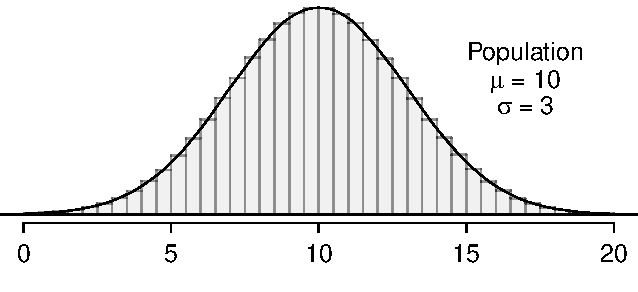
\includegraphics[width=0.55\textwidth]{ch_inference_foundations/figures/eoce/identify_dist_symm_pop/identify_dist_symm_pop.pdf} \\
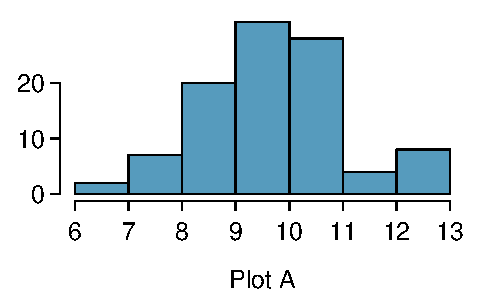
\includegraphics[width=0.325\textwidth]{ch_inference_foundations/figures/eoce/identify_dist_symm_pop/identify_dist_symm_sampling_n5.pdf}
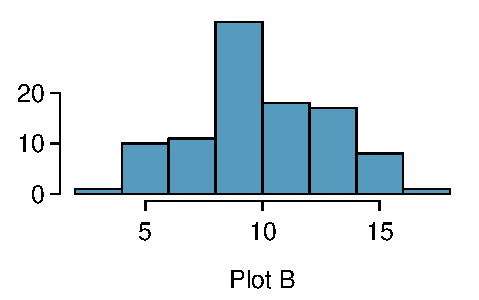
\includegraphics[width=0.325\textwidth]{ch_inference_foundations/figures/eoce/identify_dist_symm_pop/identify_dist_symm_samp.pdf}
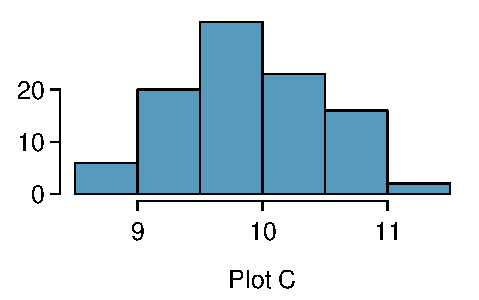
\includegraphics[width=0.325\textwidth]{ch_inference_foundations/figures/eoce/identify_dist_symm_pop/identify_dist_symm_sampling_n25.pdf}
\end{center}
}{}

\textC{\newpage}

% 38

\eoce{\qt{Identify distributions, Part II\label{identify_dist_ls_pop}} Four plots are presented below. The plot at 
the top is a distribution for a population. The mean is 60 and the standard 
deviation is 18. Also shown below is a distribution of (1) a single random 
sample of 500 values from this population, (2) a distribution of 500 sample 
means from random samples of each size 18, and (3) a distribution of 500 sample 
means from random samples of each size 81. Determine which plot (A, B, or C) is 
which and explain your reasoning.
\begin{center}
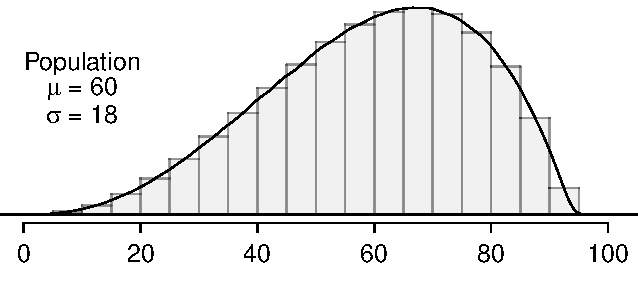
\includegraphics[width=0.55\textwidth]{ch_inference_foundations/figures/eoce/identify_dist_ls_pop/identify_dist_ls_pop.pdf}
\end{center}
\begin{center}
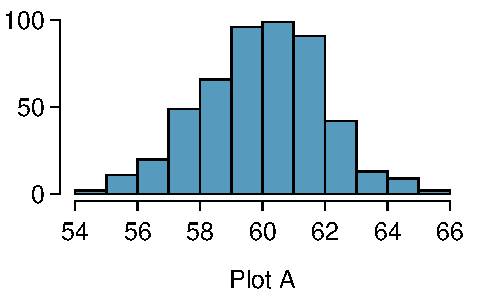
\includegraphics[width=0.325\textwidth]{ch_inference_foundations/figures/eoce/identify_dist_ls_pop/identify_dist_ls_sampling_n81.pdf}
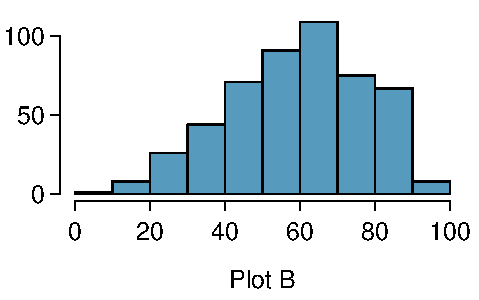
\includegraphics[width=0.325\textwidth]{ch_inference_foundations/figures/eoce/identify_dist_ls_pop/identify_dist_ls_samp.pdf}
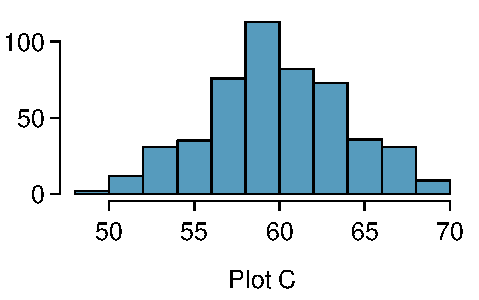
\includegraphics[width=0.325\textwidth]{ch_inference_foundations/figures/eoce/identify_dist_ls_pop/identify_dist_ls_sampling_n18.pdf}
\end{center}
}{}

% 39

\eoce{\qt{Weights of pennies\label{penny_weights}} The distribution of weights of 
United States pennies is approximately normal with a mean of 2.5 grams and a 
standard deviation of 0.03 grams.
\begin{parts}
\item What is the probability that a randomly chosen penny weighs less than 2.4 
grams?
\item Describe the sampling distribution of the mean weight of 10 randomly 
chosen pennies.
\item What is the probability that the mean weight of 10 pennies is less than 
2.4 grams?
\item Sketch the two distributions (population and sampling) on the same scale.
\item Could you estimate the probabilities from (a) and (c) if the weights of pennies had a skewed distribution?
\end{parts}
}{}

% 40

\eoce{\qt{CFLBs\label{cflbs}} A manufacturer of compact fluorescent light bulbs advertises that the 
distribution of the lifespans of these light bulbs is nearly normal with a mean 
of 9,000 hours and a standard deviation of 1,000 hours.
\begin{parts}
\item What is the probability that a randomly chosen light bulb lasts more than 
10,500 hours?
\item Describe the distribution of the mean lifespan of 15 light bulbs. 
\item What is the probability that the mean lifespan of 15 randomly chosen light 
bulbs is more than 10,500 hours?
\item Sketch the two distributions (population and sampling) on the same scale.
\item Could you estimate the probabilities from parts~(a) and~(c) if the 
lifespans of light bulbs had a skewed distribution?
\end{parts}
}{}

\textC{\pagebreak}

% 41

\eoce{\qt{Songs on an iPod\label{songs_on_ipod}} Suppose an iPod has 3,000 songs. The 
histogram below shows the distribution of the lengths of these songs. We also 
know that, for this iPod, the mean length is 3.45 minutes and the standard 
deviation is 1.63 minutes.
\begin{center}
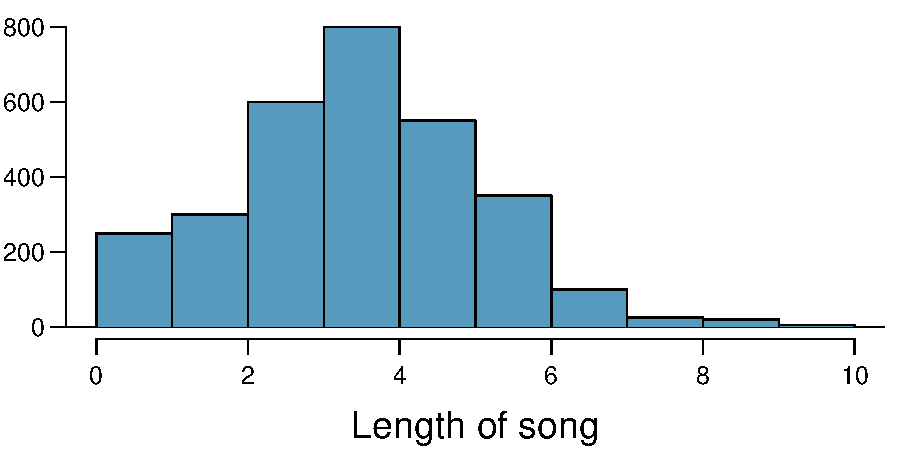
\includegraphics[width=0.5\textwidth]{ch_inference_foundations/figures/eoce/songs_on_ipod/songs_on_ipod_pop_hist.pdf}
\end{center}
\begin{parts}
\item Calculate the probability that a randomly selected song lasts more than 5 
minutes.
\item You are about to go for an hour run and you make a random playlist of 15 songs. What is the probability that your playlist lasts for the entire duration 
of your run? \textit{Hint:} If you want the playlist to last 60 minutes, what should be the minimum average length of a song?
\item You are about to take a trip to visit your parents and the drive is 6 hours. You make a random playlist of 100 songs. What is the probability that your playlist lasts the entire drive?
\end{parts}
}{}

% 42

\eoce{\qt{Spray paint\label{spray_paint}} Suppose the area that can be painted using a 
single can of spray paint is slightly variable and follows a nearly normal 
distribution with a mean of 25 square feet and a standard deviation of 3 square 
feet. 
\begin{parts}
\item What is the probability that the area covered by a can of spray paint is 
more than 27 square feet?
\item Suppose you want to spray paint an area of 540 square feet using 20 cans 
of spray paint. On average, how many square feet must each can be able to cover 
to spray paint all 540 square feet?
\item What is the probability that you can cover a 540 square feet area using 20 
cans of spray paint?
\item If the area covered by a can of spray paint had a slightly skewed 
distribution, could you still calculate the probabilities in parts~(a) and~(c) 
using the normal distribution?
\end{parts}
}{}



%_______________
\subsection{Inference for other estimators}

% 43

\eoce{\qt{Spam mail counts\label{spam_mail_count}} The 2004 National Technology 
Readiness Survey sponsored by the Smith School of Business at the University of 
Maryland surveyed 418 randomly sampled Americans, asking them how many spam 
emails they receive per day. The survey was repeated on a new random sample of 
499 Americans in 2009.\footfullcite{webpage:spam}
\begin{parts}
\item What are the hypotheses for evaluating if the average spam emails per day 
has changed from 2004 to 2009.
\item In 2004 the mean was 18.5 spam emails per day, and in 2009 this value was 
14.9 emails per day. What is the point estimate for the difference between the 
two population means?
\item A report on the survey states that the observed difference between the 
sample means is not statistically significant. Explain what this means in 
context of the hypothesis test and data.
\item Would you expect a confidence interval for the difference between the two 
population means to contain 0? Explain your reasoning.
\end{parts}
}{}

\textC{\pagebreak}

% 44

\eoce{\qt{Nearsighted\label{nearsighted}} It is believed that nearsightedness affects about 8\% of 
all children. In a random sample of 194 children, 21 are nearsighted.
\begin{parts}
\item Construct hypotheses appropriate for the following question: do these data 
provide evidence that the 8\% value is inaccurate?
\item What proportion of children in this sample are nearsighted?
\item Given that the standard error of the sample proportion is 0.0195 and the 
point estimate follows a nearly normal distribution, calculate the test 
statistic (the Z-statistic).
\item What is the p-value for this hypothesis test?
\item What is the conclusion of the hypothesis test?
\end{parts}
}{}

% 45

\eoce{\qt{Spam mail percentages\label{spam_mail_perc}} The National Technology Readiness Survey sponsored by 
the Smith School of Business at the University of Maryland surveyed 418 randomly 
sampled Americans, asking them how often they delete spam emails. In 2004, 23\% 
of the respondents said they delete their spam mail once a month or less, and in 
2009 this value was 16\%.
\begin{parts}
\item What are the hypotheses for evaluating if the proportion of those who 
delete their email once a month or less has changed from 2004 to 2009?
\item What is the point estimate for the difference between the two population 
proportions?
\item A report on the survey states that the observed decrease from 2004 to 2009 
is statistically significant. Explain what this means in context of the 
hypothesis test and the data.
\item Would you expect a confidence interval for the difference between the two 
population proportions to contain 0? Explain your reasoning.
\end{parts}
}{}

% 46

\eoce{\qt{Unemployment and relationship problems\label{unemployment_relationship}} 
A USA Today/Gallup poll conducted between 2010 and 2011 asked a group of 
unemployed and underemployed Americans if they have had major problems in their 
relationships with their spouse or another close family member as a result of 
not having a job (if unemployed) or not having a full-time job (if 
underemployed). 27\% of the 1,145 unemployed respondents and 25\% of the 675 
underemployed respondents said they had major problems in relationships as a 
result of their employment status.
\begin{parts}
\item What are the hypotheses for evaluating if the proportions of unemployed and underemployed people who had relationship problems were different?
\item The p-value for this hypothesis test is approximately 0.35. Explain what this means in context of the hypothesis test and the data.
\end{parts}
}{}

% 47

\eoce{\qt{Practical vs. statistical\label{prac_stat_sig}} Determine whether the 
following statement is true or false, and explain your reasoning: ``With large 
sample sizes, even small differences between the null value and the point 
estimate can be statistically significant."
}{}

% 48

\eoce{\qt{Same observation, different sample size\label{same_obs_diff_n}} Suppose you 
conduct a hypothesis test based on a sample where the sample size is $n = 50$, 
and arrive at a p-value of 0.08. You then refer back to your notes and discover 
that you made a careless mistake, the sample size should have been $n = 500$. 
Will your p-value increase, decrease, or stay the same? Explain.
}{}
